\scanpage{134}
U N I V E R S I T E\\
DES SCIENCES ET TECHNIQUES\\
DU LANGUEDOC\\
\texttt{------------}

Montpellier, le 25 Novembre 1981

Service de la Scolarité\\
MA / GJ\\
Diffusion : Liste A\\
N° 6443

AVIS DE SOUTENANCE D'UNE THESE DE DOCTORAT DE SPECIALITE

MATHEMATIQUES APPLIQUEES\\
\texttt{------------------------}

\uline{Nom et prénom du candidat} : ROS Marius

\uline{Titre de la thèse} : Sur quelques questions de cinématique et de statique des surfaces.

\uline{Date, heure et lieu de soutenance prévus} :\\
10 DECEMBRE 1981 à 10 Heures\\
Salle 431 - Bâtiment des Mathématiques - USTL

\uline{Nom du Directeur de thèse} : Monsieur le Professeur MOREAU

\uline{Désignation du laboratoire où la thèse est préparée} : Mathématiques

\uline{Résumé de la thèse} :

Une membrane étant représentée par une surface différentiable, on étudie les conditions pour qu'un champ tensoriel symétrique soit le champ tensoriel des vitesses de déformation. Localement, tout champ tensoriel symétrique suffisamment différentiable peut être considéré comme un champ tensoriel des vitesses de déformation si la surface est localement, de type hyperbolique, elliptique ou parabolique ; cela n'est plus vrai dans le cas localement plan. Globalement, des théorèmes d'unicité pour le champ vectoriel des vitesses correspondant sont obtenus dans le cas des surfaces simplement connexes de type hyperbolique ou elliptique. Ceci entraîne la rigidité de certaines membranes en mouvement isométrique dont le bord est rigide. Un résultat corré-\\
latif est que, pour une membrane de même forme, en équilibre en l'absence de forces extérieures, le champ tensoriel des contraintes est nul.

\uline{Durée approximative des recherches ayant abouti à la thèse} : 4 ans

\uline{Composition du jury proposé} :\\
MM. MOREAU J.-J.\\
JOUANNA P.\\
MAISONNEUVE O.

P. le Secrétaire Général,\\
L'Attachée d'Administration Universitaire,

\figure{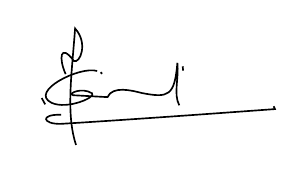
\begin{tikzpicture}[x=0.004cm,y=-0.004cm,line width=0.6pt]
\draw (678,430) .. controls (645,330) and (665,200) .. (675,60)
 .. controls (718,107) and (690,173) .. (671,163)
 .. controls (628,105) and (622,154) .. (645,205);
\draw (745,195) .. controls (691,178) and (527,260) .. (600,296)
 .. controls (650,319) and (743,278) .. (729,266)
 .. controls (698,245) and (648,267) .. (669,272)
 -- (778,278) .. controls (794,241) and (856,257) .. (887,265)
 .. controls (971,281) and (991,276) .. (1000,169)
 .. controls (1005,219) and (987,269) .. (1006,304);
\draw (1017,180)--(1018,194);
\draw (756,199)--(761,204);
\draw (569,281)--(580,301);
\draw (631,334) .. controls (562,332) and (572,364) .. (629,363)
 .. controls (842,350) and (1104,331) .. (1310,316)--(1306,307);
\end{tikzpicture}}
A. GENTIL

\mspage{133}
